%%
%% This is file `tikzposter-template.tex',
%% generated with the docstrip utility.
%%
%% The original source files were:
%%
%% tikzposter.dtx  (with options: `tikzposter-template.tex')
%%
%% This is a generated file.
%%
%% Copyright (C) 2014 by Pascal Richter, Elena Botoeva, Richard Barnard, and Dirk Surmann
%%
%% This file may be distributed and/or modified under the
%% conditions of the LaTeX Project Public License, either
%% version 2.0 of this license or (at your option) any later
%% version. The latest version of this license is in:
%%
%% http://www.latex-project.org/lppl.txt
%%
%% and version 2.0 or later is part of all distributions of
%% LaTeX version 2013/12/01 or later.
%%


\documentclass{tikzposter} %Options for format can be included here

\usepackage{todonotes}

\usepackage[tikz]{bclogo}
\usepackage{lipsum}
\usepackage{amsmath}
\usepackage{fontawesome}
\usepackage{booktabs}
\usepackage{longtable}
\usepackage[absolute]{textpos}
\usepackage[it]{subfigure}
\usepackage{graphicx}
\usepackage{cmbright}
%\usepackage[default]{cantarell}
%\usepackage{avant}
%\usepackage[math]{iwona}
\usepackage[math]{kurier}
\usepackage[T1]{fontenc}
\usepackage{tikz}
%% add your packages here
\usepackage{hyperref}
% for random text
\usepackage{lipsum}
\usepackage[english]{babel}
\usepackage[pangram]{blindtext}

\usepackage{forest}
%\usetikzlibrary{arrows.meta, shapes.geometric, calc, shadows}

\usepackage[utf8]{inputenc}
\usepackage{dtk-logos}
\usepackage{tikz}

\usetikzlibrary{arrows,chains,mindmap,shadows,automata,patterns,petri,shapes.geometric,shapes.misc, spy, trees,decorations.markings}
%\usepackage[hidelinks,pdfencoding=auto]{hyperref}
% Information boxes
\newcommand*{\info}[4][4]{%
  \node [ annotation, #3, text width = 3.5cm,
          inner sep = 0.3em ] at (#2) {%
  \list{$\bullet$}{\topsep=-3pt\itemsep=0pt\parsep=1pt
    \parskip=1pt\labelwidth=0pt\leftmargin=1pt
    \itemindent=1pt\labelsep=1pt}%
    #4
  \endlist
  };
}

%forest
\usepackage{forest}
\usetikzlibrary{arrows.meta, shapes.geometric, calc, shadows}
\colorlet{mygreen}{green!75!black}
\colorlet{col1in}{red!30}
\colorlet{col1out}{red!40}
\colorlet{col2in}{mygreen!40}
\colorlet{col2out}{mygreen!50}
\colorlet{col3in}{blue!30}
\colorlet{col3out}{blue!40}
\colorlet{col4in}{mygreen!20}
\colorlet{col4out}{mygreen!30}
\colorlet{col5in}{blue!10}
\colorlet{col5out}{blue!20}
\colorlet{col6in}{blue!20}
\colorlet{col6out}{blue!30}
\colorlet{col7out}{orange}
\colorlet{col7in}{orange!50}
\colorlet{col8out}{orange!40}
\colorlet{col8in}{orange!20}
\colorlet{linecol}{blue!60}

\colorlet{backgroundcolor}{blue!10}


 % Title, Author, Institute
\title{Team for Universal Learning and Intelligent Processing}
\author{Gang Li}
\institute{$^1$ School of Information Technology \\
	            Deakin University, Australia
}
%\titlegraphic{logos/tulip-logo.eps}

%Choose Layout
\usetheme{Wave}

%\definebackgroundstyle{samplebackgroundstyle}{
%\draw[inner sep=0pt, line width=0pt, color=red, fill=backgroundcolor!30!black]
%(bottomleft) rectangle (topright);
%}
%
%\colorlet{backgroundcolor}{blue!10}

\begin{document}


\colorlet{blocktitlebgcolor}{blue!23}

 % Title block with title, author, logo, etc.
\maketitle

\begin{columns}
 % FIRST column
\column{0.5}% Width set relative to text width

%%%%%%%%%% -------------------------------------------------------------------- %%%%%%%%%%
 %\block{Main Objectives}{
%  	      	\begin{enumerate}
%  	      	\item Formalise research problem by extending \emph{outlying aspects mining}
%  	      	\item Proposed \emph{GOAM} algorithm is to solve research problem
%  	      	\item Utilise pruning strategies to reduce time complexity
%  	      	\end{enumerate}
%%  	      \end{minipage}
%}
%%%%%%%%%% -------------------------------------------------------------------- %%%%%%%%%%


%%%%%%%%%% -------------------------------------------------------------------- %%%%%%%%%%
\block{TULIP Lab}{
\selectcolormodel{rgb}
\pgfkeys{/forest,
  rect/.append style   = { rounded corners = 2pt,
                         inner color = col6in, outer color = col6out},
  ellip/.append style  = { inner color = col5in,
                          outer color = col5out},
  orect/.append style  = { font = \sffamily\bfseries\LARGE,
                         text width = 325pt, text centered,
                         minimum height = 10pt, outer color = col7out,
                         inner color=col7in},
  oellip/.append style = { inner color = col8in, outer color = col8out,
                          font = \sffamily\bfseries\large, text centered}}
\begin{forest}
  for tree={
      font=\sffamily\bfseries,
      line width=1pt,
      draw=linecol,
      ellip,
      align=center,
      child anchor=north,
      parent anchor=south,
      drop shadow,
      l sep+=12.5pt,
      edge path={
        \noexpand\path[color=linecol, rounded corners=5pt,
          >={Stealth[length=11pt]}, line width=1pt, ->, \forestoption{edge}]
          (!u.parent anchor) -- +(0,-5pt) -|
          (.child anchor)\forestoption{edge label};
        },
      where level={3}{tier=tier3}{},
      where level={0}{l sep-=5pt}{},
      where level={1}{}{},
  }
    [TULIP Academy %inner color=col1in, outer color=col1out
    [Visitor]
    [Flipper
    [Trainee
        [[FLIP (00)]
          [\dots]
          [FLIP (05)]
        ]
    ]]
    [TULIP Lab
        [Australia]
        [China]
        [India]]
    [Alumni] %inner color =col7in, outer color = col7out]
    [Web Team] %, inner color=col2in, outer color=col2out]
  ]
\end{forest}
  	
\begin{description}
\item[Official Websites]
  \begin{itemize}
    \item \textcolor{orange}{\faHome:} \url{http://www.tulip.org.au}
    \item \textcolor{orange}{\faGithub:} \url{https://github.com/tulip-lab}
  \end{itemize}

\item[Social Media]
  \begin{itemize}
    \item \textcolor{orange}{\faTwitter:} \href{https://twitter.com/tulipacademy}{tulipacademy}
    \item \textcolor{orange}{\faWeibo:} \href{https://weibo.com/tulipacademy}{tulipacademy}
    \item \textcolor{orange}{\faRedditAlien:} \url{https://www.reddit.com/r/tulipacademy}
  \end{itemize}


\item[Internal Services]
  \begin{itemize}
   \item \textcolor{orange}{\faBitbucket:} \url{https://bitbucket.org}
   \item \textcolor{orange}{\faCalendar:} \url{https://goo.gl/cWCWwC}
   \item \textcolor{orange}{\faCalendarCheckO:} \url{https://goo.gl/aC9VWW} (iCal)
  \end{itemize}

\end{description}
}
%%%%%%%%%% -------------------------------------------------------------------- %%%%%%%%%%


%%%%%%%%%% -------------------------------------------------------------------- %%%%%%%%%%
\block{Research mind map}{

\begin{minipage}{0.9\linewidth}
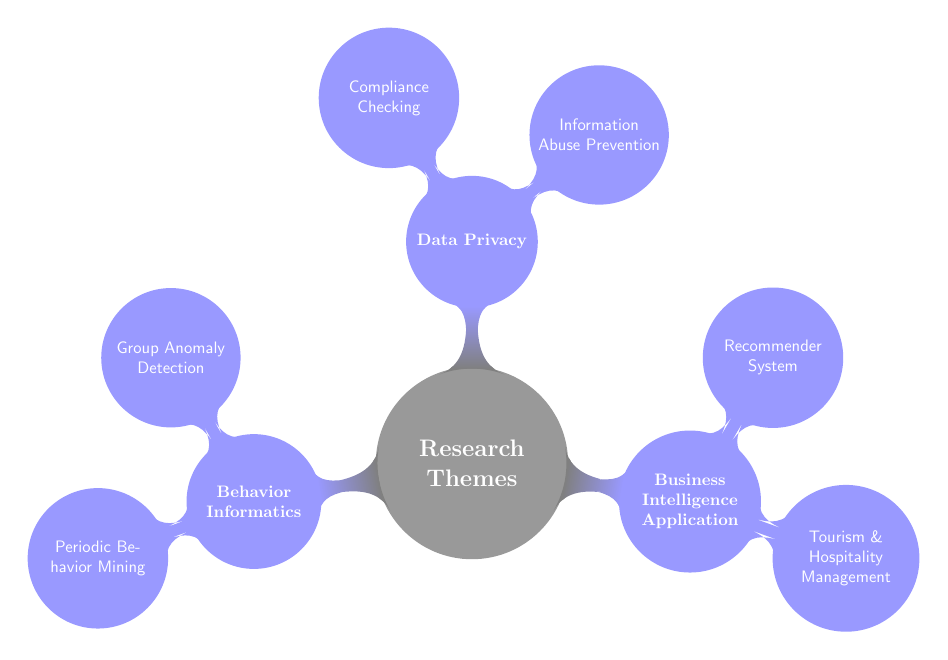
\begin{tikzpicture}[ every annotation/.style = {draw,
                     fill = white}]
  \path[mindmap,concept color=black!50,text=white,
    every node/.style={concept},
    root/.style    = {concept color=black!40,
      font=\Large\bfseries,text width=10em},
    level 1 concept/.append style={font=\bfseries,
      sibling angle=100,text width=7.7em,level distance=8em,inner sep=0pt},
    level 2 concept/.append style={font=\sf,sibling angle=80,text width=8em,inner sep=0pt,level distance=6em},
  ]
  node[root,scale=0.6, text=white] {Research Themes} [clockwise from=190]
    child[concept color=blue!40] {
      node[scale=0.6] {Behavior Informatics} [clockwise from=200]
        child { node[scale=0.6] (pbm){Periodic Behavior Mining}}
        child { node[scale=0.6] (bp) {Group Anomaly Detection}}
    }
     child[concept color=blue!40] {
      node[concept,scale=0.6] {Data Privacy}[clockwise from=120]
      child{node[concept,scale=0.6](dcc){Compliance Checking}}
      child{node[concept,scale=0.6](privacy){Information Abuse Prevention}}
    }
    child[concept color=blue!40] {
      node[concept,scale=0.6] {Business Intelligence Application}[clockwise from=60]
      child{node[concept,scale=0.6](rs){Recommender System} }
      child{node[concept,scale=0.6](t/hm){Tourism \& Hospitality Management}}
    }
;
\end{tikzpicture}

\end{minipage}

}
%%%%%%%%%% -------------------------------------------------------------------- %%%%%%%%%%

%%%%%%%%%% -------------------------------------------------------------------- %%%%%%%%%%
\block{Traning Mind Map}{
\begin{center}
\scalebox{0.9}{
\setlength{\abovecaptionskip}{-15pt}
\selectcolormodel{rgb}
   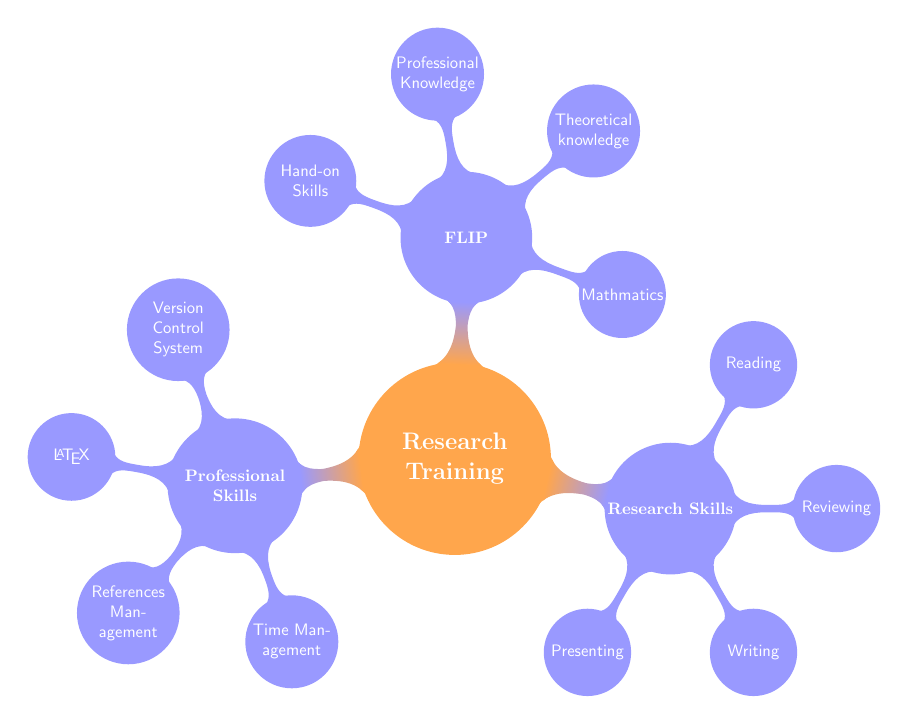
\begin{tikzpicture}[ every annotation/.style = {draw,
                     fill = white}]
  \path[mindmap,concept color=orange!70,text=white,
    every node/.style={concept},
    root/.style    = {concept color=orange!70,
      font=\Large\bfseries,text width=9em},
    level 1 concept/.append style={font=\bfseries,
      sibling angle=100,text width=7.7em,level distance=8em,inner sep=0pt},
    level 2 concept/.append style={font=\sf,text width=5em,inner sep=0pt, level distance=6em},
  ]
  node[root,scale=0.6, text=white] {Research Training} [clockwise from=187]
    child[concept color=blue!40] {
      node[scale=0.6] {Professional Skills} [clockwise from=290]
        child { node[scale=0.6] (goReview) {Time Management}}
        child { node[scale=0.6] (goRefrences ){References Management}}
        child { node[scale=0.6] {\LaTeX}}
        child { node[scale=0.6] (goVersionCon) {Version Control System}}
    }
     child[concept color=blue!40] {
      node[concept,scale=0.6] {FLIP}[clockwise from=160]
      child{node[concept,scale=0.6](hand-on){Hand-on Skills}}
      child{node[concept,scale=0.6](Professional){Professional Knowledge}}
      child{node[concept,scale=0.6](Theo){Theoretical knowledge}}
      child{node[concept,scale=0.6](Math){Mathmatics}}
    }
    child[concept color=blue!40] {
      node[concept,scale=0.6] {Research Skills}
        [clockwise from=60]
      child { node[concept,scale=0.6] (TeXampleBlog){Reading}}
      child { node[concept,scale=0.6] (Reviewteam){Reviewing}}
      child { node[concept,scale=0.6] (present){Writing}}
      child { node[concept,scale=0.6] (write){Presenting}}
    }
   ;
    \end{tikzpicture}}
\end{center}
}
%%%%%%%%%% -------------------------------------------------------------------- %%%%%%%%%%


%%%%%%%%%% -------------------------------------------------------------------- %%%%%%%%%%

%\note{Note with default behavior}

%\note[targetoffsetx=12cm, targetoffsety=-1cm, angle=20, rotate=25]
%{Note \\ offset and rotated}

 % First column - second block
\column{0.5}

%%%%%%%%%% -------------------------------------------------------------------- %%%%%%%%%%
\block{Research @ TULIP -   Theme 2.Data Privacy}{

%\begin{description}
	\begin{itemize}
		\item
		{Information Abuse}
 			 \begin{itemize}
   				 \item The compromise of information for which the data stakeholders are not willing to disclose.
				 \item It depends on the nature of the information, the involved internal or external users, and the ways in which the organization rants the access to or releases the information.
				 \item Every user is potentially an adversary. Once the data is released, we cannot prevent any user from performing any type of analysis on it.
		 		%The worst case scenario is that we must account for disclosure risk from any and all types of analyses.	
  			\end{itemize}
	
%\end{description}
\vspace{.2cm}

\item
Case Study

\begin{enumerate}
	\item
  	Is O.S.N. a Secure Place to Show off?
	\vspace{.1cm}
	
  	\begin{minipage}{0.69\linewidth}	
		\centering
		\textbf{\large{\textcolor{orange}{Did Facebook photo trigger murder?}}}	
		\vspace{.1cm}
		\begin{description}
			\item
			{\textcolor{blue!60}{Aubrey Whelan, INQUIRER STAFF WRITER\\
			LAST UPDATED: Tuesday, October 13, 2015, 5:18 PM\\
			POSTED: Tuesday, October 13, 2015, 7:26 AM}}
		\end{description}		
	\end{minipage}	
  	\begin{minipage}{0.3\linewidth}
 	 	\begin{tikzfigure}
			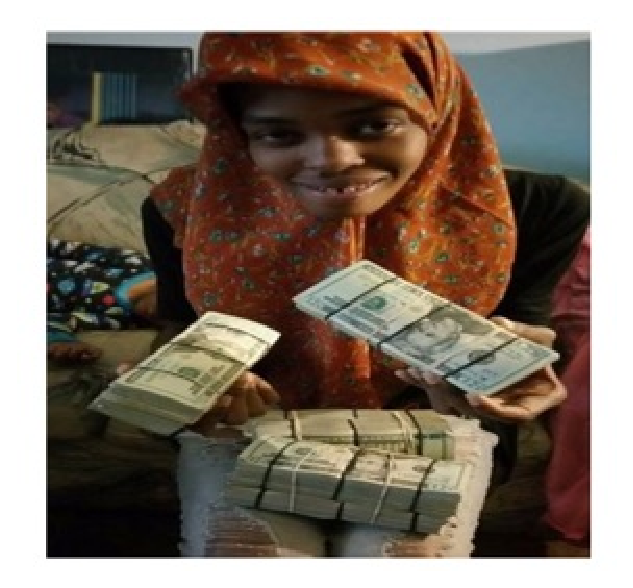
\includegraphics[scale=0.7]{./figures/theme2/case3_1.eps}
		 \end{tikzfigure}
	\end{minipage}	
	
	\fbox{
	\centering

	\parbox{0.95\linewidth}{
		\small{
		\begin{description}
			\item Last week,Tony Harris, a 50-year-old electronics repairman, uploaded a photo to his Facebook page - something different from his standard fare of videos and memes and images of his three children.
		\end{description}
		\begin{description}
			\item This one showed his wife, Amber Crane grinning up at the camera, clutching thick stacks of cash in both hands. More money sat piled in her lap.
		\end{description}
		\begin{description}
			\item ``I misplaced \$60,000.00. I hope my wife didn't go shopping with it,'' the caption joked.
		\end{description}
		\begin{description}
			\item ``Stop playing,''a friend wrote back.
		\end{description}
		\begin{description}
			\item Precisely a week later about 11:30 at night, police said three young people walked into his home on the 1100 block of South Ruby Street in Kingsessing, where he has lived for decades.
		\end{description}
		}}
	}

	\vspace{.2cm}
	
  	\item
 	Privacy Breach
 	 \vspace{.1cm}
% 	 \begin{description}
%    		\item
%		\centering	
%    		Privacy breach of Singapore residents traveling overseas
% 		 \end{description}
% 	 \begin{minipage}{\linewidth}
%  		\centering
%  		\fontsize{24pt}{24pt}\selectfont
% 		 \begin{tabular}{c|c|l|l|c|c}	
%			\toprule
%			ID  	&  	\textbf{User(Gender)}		& 		\textbf{Visited Destination} 		& 		\textbf{Venue} 		& 	\textbf{Date} 		&	\textbf{Time}	\\
%			\midrule	
%			$L_1$	&	$U_5$(M)-$U_6$(F)	&	Shanghai, China 	   &	UNCO Lounge		&	25-May-2015	&	20:17\\
%			$L_2$	&	$U_5$(M)-$U_6$(F)	&	Shanghai, China 	   &	T8 Restaurant and Bar		&	26-May-2015	&	17:35\\
%			$L_3$	&	$U_5$(M)-$U_6$(F)	&	Cannes, France 	       &	Villa Mystique Resort		&	25-Jun-2015	&	11:03\\	
%			$L_4$	&	$U_5$(M)-$U_6$(F)	&	Paris, France 		   &	Dersou Restaurant			&	27-Jun-2015	&	19:58\\
%			$L_5$	&	$U_5$(M)-$U_6$(F)	&	Paris, France 		   &	Ladure Pastry Shop			&	28-Jun-2015	&	14:48\\
%			$L_6$	&	$U_5$(M)-$U_6$(F)	&	London, United Kingdom &	L'ETO Caff			&	10-Oct-2015	&	11:01\\
%			$L_7$	&	$U_5$(M)-$U_6$(F)	&	Hong Kong		       &	The Ocean Club Bar			&	31-Oct-2015	&	18:47\\
%			$L_8$	&	$U_5$(M)-$U_6$(F)	&	Hanoi, Vietnam		   &	HOME Hanoi Restaurant			&	01-Jan-2016	&	19:04\\
%			$L_9$	&	$U_5$(M)-$U_6$(F)	&	Ho Chi Minh, Vietnam   &	MGallery Hotel des Art		&	30-Jun-2016	&	19:54\\
%			$L_{10}$	&	$U_5$(M)-$U_6$(F)	&	Ho Chi Minh, Vietnam   &	L'Usine: Cafe		&	01-Jul-2016	&	10:55\\
%			$L_{11}$	&	$U_5$(M)-$U_6$(F)	&	Ho Chi Minh, Vietnam   &	Social Club @ Hotel Des Arts		&	01-Jul-2016	&	17:04\\
%			\bottomrule
% 		 \end{tabular}
%  	\end{minipage}
  	\vspace{.1cm}
 	 \begin{description}
   		 \item
		 \centering
    		Joint check-in record indicating sensitive contrast relationship
  	 \end{description}
  	 \begin{minipage}{\linewidth}
  		 \centering
 		  \fontsize{24pt}{24pt}\selectfont
  		 \begin{tabular}{c | c  | p{9cm} | p{6cm}  | p{3cm}}	
			\toprule	
			ID  	&  	\textbf{User(Gender)}& 	\textbf{Venue} 		& 	\textbf{Date} 	&	\textbf{Time}	\\
			\midrule
			$C_1$	&	$U_9$(M)-$U_{10}$(F)	 &	Zouk Night Club		&	11-Sep-2015	    &	23:31\\
			$C_2$	&	$U_9$(M)-$U_{11}$(F)	 &	Zouk Night Club		&	18-Nov-2015	    &	23:50\\
			$C_3$	&	$U_9$(M)-$U_{11}$(F)	 &	Club Luxi			&	17-Jan-2016	    &	00:30\\
			$C_4$	&	$U_9$(M)-$U_{11}$(F)	 &	Club Hollywood		&	06-Feb-2016     &	04:34\\
			$C_5$	&	$U_9$(M)-$U_{10}$(F)	 &	Wave House Sentosa	&	12-Mar-2016	    &	22:43\\
			$C_6$	&	$U_9$(M)-$U_{10}$(F)	 &	Zouk Night Club		&	02-Jul-2016	    &	00:25\\
			$C_7$	&	$U_9$(M)-$U_{10}$(F)	 &	Zouk Night Club		&	07-Aug-2016	    &	00:39\\
			\bottomrule
  		 \end{tabular}
  	 \end{minipage}
\end{enumerate}

\end{itemize}
}
%%%%%%%%%% -------------------------------------------------------------------- %%%%%%%%%%


% SECOND column

 %Second column with first block's top edge aligned with with previous column's top.

%%%%%%%%%% -------------------------------------------------------------------- %%%%%%%%%%
\block{Research @ TULIP -   Theme 3. Business Intelligence}{


\begin{itemize}
		\item Tourism Data Mining
		
		\begin{itemize}
			\item Tourist Behavior Analysis
			
			\item Contrast Mining
			
			\begin{itemize}
				
				\item Outlying Aspects Mining
				
				\item Competitiveness Discovery
				
			\end{itemize}
			
		\end{itemize}
		
		\item Recommendation System
		\begin{itemize}
			\item Group package recommendation
			\item Heterogeneous Preferences
		\end{itemize}
		
  \item Case Study


    \begin{enumerate}
      \item
      Case Study(1). Market Segmentation Analysis

      \item
      Case Study(2). Negative Association Rule Mining

      \item
      Case Study(3). Contrast Mining

      \item
      Case Study(4). PR Based Conditional Random Fields

    \end{enumerate}
\end{itemize}


}
%%%%%%%%%% -------------------------------------------------------------------- %%%%%%%%%%
% Second column - first block


%%%%%%%%%% -------------------------------------------------------------------- %%%%%%%%%%
\block[titleleft]{Awards}
{
\begin{minipage}{\linewidth}
%\begin{table}[htbp]
%  \centering
 %  \caption{TULIP Lab Research Awards}
\begin{tabular}{ r | l | r  r }
\toprule
\multicolumn{1}{ l |}{\textbf{Year}} & \textbf{Awards} & \textbf{Author} &  \\
\midrule
\textbf{2018} & KSEM 2018 \textit{Best Paper} Award & Shaoni Wang &  \\

\textbf{2017} & IFITT \textit{Journal Paper of The Year} Award (1st Prize) & Huy Quan Vu &  \\

\textbf{2016} & IEEE TrustCom 2016 \textit{Best Student Paper} Award & Na Pang &  \\

\textbf{2015} & IFITT \textit{Journal Paper of The Year} Award (3rd Prize) & Huy Quan Vu &  \\

\textbf{2014} & PAKDD 2014 \textit{Best Student Paper} Award & Tianqing Zhu &  \\

\textbf{2012} & ACM ASONAM 2012  \textit{Best Paper} Award & Yongli Ren &  \\

\textbf{2007} & Springer 2007 \textit{Nightingale Prize} & Jingyu Hou &  \\
\bottomrule
\end{tabular}
%\end{table}
\end{minipage}
}
%%%%%%%%%% -------------------------------------------------------------------- %%%%%%%%%%


% Second column - second block
%%%%%%%%%% -------------------------------------------------------------------- %%%%%%%%%%
\block[titlewidthscale=1, bodywidthscale=1]
{Training @ TULIP}
{
%\begin{center}
%\selectcolormodel{rgb}
%\smartdiagramset{description title width=2cm,
%set color list={blue!40,blue!30,orange!40},
%description title text width=1.75cm,
%descriptive items y sep=3.5cm,
%description text width=12cm,
%module minimum height=.4cm}
%
%\smartdiagram[descriptive diagram]{
%{\textbf{$\infty$}, \begin{enumerate}
%         \item Proactively meet with supervisor twice per week
%         \item Proactively present and criticize at \textit{TULIP Seminar}
%         \item FLIP (04-05) and FLIP (06-07) completion
%         \item Act as FLIP team leaders and update materials annually
%         \end{enumerate}},
%{\textbf{Trainee}, \begin{enumerate}
%         \item FLIP (02-03) with success on open \href{https://www.kaggle.com}{Kaggle} projects
%         \item Feedback and suggestions on FLIP
%         \item Present at \textit{TULIP Seminar}
%         \end{enumerate}},
%{\textbf{Flipper},\begin{enumerate}
%         \item \LaTeX + \faGithub \faBitbucket + Time management + PPR skill
%		 \item Keep FLIP materials confidential without distribution
%         \item FLIP (00-01) with success on open \href{https://www.kaggle.com}{Kaggle} projects
%         \item Attend \textit{TULIP Seminar} with preparation and questions
%         \end{enumerate}},}
%\end{center}
}
%%%%%%%%%% -------------------------------------------------------------------- %%%%%%%%%%


% Bottomblock
%%%%%%%%%% -------------------------------------------------------------------- %%%%%%%%%%
\colorlet{notebgcolor}{blue!20}
\colorlet{notefrcolor}{blue!20}
\note[targetoffsetx=8cm, targetoffsety=-4cm, angle=30, rotate=15,
radius=2cm, width=.26\textwidth]{
Acknowledgement
\begin{itemize}
    \item
    International Cooperation Project (Y7Z0511101)
    of IIE,
    Chinese Academy of Sciences
 \end{itemize}
}

%\note[targetoffsetx=8cm, targetoffsety=-10cm,rotate=0,angle=180,radius=8cm,width=.46\textwidth,innersep=.1cm]{
%Acknowledgement
%}

%\block[titlewidthscale=0.9, bodywidthscale=0.9]
%{Acknowledgement}{
%}
%%%%%%%%%% -------------------------------------------------------------------- %%%%%%%%%%

\end{columns}


%%%%%%%%%% -------------------------------------------------------------------- %%%%%%%%%%
%[titleleft, titleoffsetx=2em, titleoffsety=1em, bodyoffsetx=2em,%
%roundedcorners=10, linewidth=0mm, titlewidthscale=0.7,%
%bodywidthscale=0.9, titlecenter]

%\colorlet{noteframecolor}{blue!20}
\colorlet{notebgcolor}{blue!20}
\colorlet{notefrcolor}{blue!20}
\note[targetoffsetx=-13cm, targetoffsety=-12cm,rotate=0,angle=180,radius=8cm,width=.96\textwidth,innersep=.4cm]
{
\begin{minipage}{0.3\linewidth}
\centering

\includegraphics[width=24cm]{logos/tulip-wordmark.eps}
\end{minipage}
\begin{minipage}{0.7\linewidth}
{ \centering
 \large{\textcolor{blue!80}{Welcome to \emph{Team for Universal Learning and
 Intelligent Processing}!}}
}
\end{minipage}
}
%%%%%%%%%% -------------------------------------------------------------------- %%%%%%%%%%


\end{document}

\endinput
%%
%% End of file `tikzposter-template.tex'.
